

\chapter{Inngangur að rafrásum}

\section{Íhlutir í rafrásir}

\begin{table}[ht]
  \centering
  \begin{tabular}{ | c | l | c |}
    \hline
    Mynd & Lýsing & Tákn \\ \hline \hline
    \begin{minipage}{.3\textwidth}
    \vspace{0.3cm}
    \centering
        \begin{circuitikz}[american voltages]
        \draw (0,0) to[battery1=\,, o-o] (2,0);
    \end{circuitikz}
    \vspace{0.3cm}
    \end{minipage}
    &
      Rafhlaða & $V$
    \\ \hline
    
    \begin{minipage}{.3\textwidth}
    \vspace{0.3cm}
    \centering
        \begin{circuitikz}
        \draw (0,0) to[short, i = $I$, o-o] (2,0);
    \end{circuitikz}
    \vspace{0.3cm}
    \end{minipage} 
    &
    Rafstraumur & $I$
    \\ \hline
    
    \begin{minipage}{.3\textwidth}
    \vspace{0.3cm}
    \centering
        \begin{circuitikz}
        \draw (0,0) to[R, o-o] (2,0);
    \end{circuitikz}
    \vspace{0.3cm}
    \end{minipage} 
    &
    Viðnám & $R$
    \\ \hline
    
    
   \begin{minipage}{.3\textwidth}
    \vspace{0.3cm}
    \centering
        \begin{circuitikz}
        \draw (0,0) to[C, o-o] (2,0);
    \end{circuitikz}
    \vspace{0.3cm}
    \end{minipage}
    &
      Þéttir & $C$
    \\ \hline
    
    \begin{minipage}{.3\textwidth}
    \vspace{0.3cm}
    \centering
        \begin{circuitikz}
        \draw (0,0) to[L, o-o] (2,0);
    \end{circuitikz}
    \vspace{0.3cm}
    \end{minipage}
    & 
    Spóla & $L$
    \\ \hline
    
    \begin{minipage}{.3\textwidth}
    \vspace{0.3cm}
    \centering
        \begin{circuitikz}[american voltages]
        \draw (0,0) to[sinusoidal voltage source=\,, o-o] (2,0);
    \end{circuitikz}
    \vspace{0.3cm}
    \end{minipage}
    & 
    Riðspennugjafi & $\mathcal{E}(t)$
    \\ \hline
  \end{tabular}
  \caption{Íhlutir í rafrásum sem hafa algebrulegar stærðir.} 
  \label{table:rafrasarihlutir1}
\end{table}

\begin{table}[h!]
  \centering
  \begin{tabular}{ | c | l | }
    \hline
    Mynd & Lýsing \\ \hline \hline
    
    \begin{minipage}{.3\textwidth}
    \vspace{0.3cm}
    \centering
        \begin{circuitikz}
        \draw (0,0) to[short,o-] (1,0) node[ground] {} to[short,-o] (2,0);
    \end{circuitikz}
    \vspace{0.3cm}
    \end{minipage}
    & 
    Jarðtenging
    \\ \hline

    
        \begin{minipage}{.3\textwidth}
    \vspace{0.3cm}
    \centering
        \begin{circuitikz}
        \draw (0,0) to[normal open switch, o-o] (2,0);
    \end{circuitikz}
    \vspace{0.3cm}
    \end{minipage}
    &
      
    Rofi
    \\ \hline
    
    \begin{minipage}{.3\textwidth}
    \vspace{0.3cm}
    \centering
        \begin{circuitikz}
        \draw (0,0) to[bulb, o-o] (2,0);
    \end{circuitikz}
    \vspace{0.3cm}
    \end{minipage}
    &
    Ljósapera
    \\ \hline
    
            \begin{minipage}{.3\textwidth}
    \vspace{0.3cm}
    \centering
        \begin{circuitikz}
        \draw (0,0) to[rmeter, t=$V$, o-o] (2,0);
    \end{circuitikz}
    \vspace{0.3cm}
    \end{minipage}
    &
    Spennumælir
    \\ \hline
    
    \begin{minipage}{.3\textwidth}
    \vspace{0.3cm}
    \centering
        \begin{circuitikz}
        \draw (0,0) to[rmeter, t=$A$, o-o] (2,0);
    \end{circuitikz}
    \vspace{0.3cm}
    \end{minipage}
    & 
    Straummælir
    \\ \hline
    
    \begin{minipage}{.3\textwidth}
    \vspace{0.3cm}
    \centering
        \begin{circuitikz}
        \draw (0,0) to[rmeter, t=$\Omega$, o-o] (2,0);
    \end{circuitikz}
    \vspace{0.3cm}
    \end{minipage}
    & 
    Viðnámsmælir
    \\ \hline

  \end{tabular}
  \caption{Aðrir algengir íhlutir í rafrásir.} \label{table:rafrasarihlutir}
\end{table}

\begin{comment}
Til þess að tákna einhvern ótiltekinn íhlut (hvað sem er í töflunni fyrir ofan) í rafrás notum við:
\begin{figure}[H]
    \centering
    \begin{circuitikz}
        \draw (0,0) to[transmission line, o-o] (2,0);
    \end{circuitikz}
\end{figure}
\end{comment}

\section{Lögmál Kirchoffs}

\begin{tcolorbox}
\begin{theorem}
Við höfum eftirfarandi tvö lögmál fyrir rafrásir:
\begin{enumerate}[label = \textbf{(\roman*)}]
    \item \textbf{(Gatnamótalögmál Kirchoffs)} Rafstraumsflæðið er varðveitt. Það er að segja við höfum í sérhverjum punkti að:
    \begin{align*}
        I_{\text{inn}} = I_{\text{út}}
    \end{align*}
    \item \textbf{(Lykkjulögmál Kirchoffs)} Sspennufallið í gegnum lykkju í rafrás er núll. Þ.e.a.s.~
    \begin{align*}
       \Delta V_{\text{lykkja}} = \Delta V_1 + \Delta V_2 + \ldots + \Delta V_n = 0
    \end{align*}
\end{enumerate}
\end{theorem}
\begin{figure}[H]
    \centering
    \begin{tikzpicture}
    \draw (0,0) to[short, i = $I_{\text{inn}}$] (2,0)
    (2,0) to[short, i = $I_1$] (2,1) to (4,1)
    (2,0) to[short, i = $I_2$] (4,0)
    (2,0) to[short, i = $I_3$] (2,-1) to (4,-1)
    ;
    \draw (6,1) to[transmission line, l = $\Delta V_1$] (9,1) to[transmission line, l = $\Delta V_2$] (9,-1) to[transmission line, l = $\Delta V_3$] (6,-1) to[transmission line, l = $\Delta V_4$] (6,1)
    ;
    \draw[thin, <-, >=triangle 45] (7.5,0)node{}  ++(-60:0.5) arc (-60:170:0.5);
    \end{tikzpicture}
\end{figure}
\end{tcolorbox}

\textbf{Útleiðsla:} Gatnamótalögmálið er afleiðing af því að rafflæði er varðveitt (samanber vatnsflæði í vatnspípum). Lykkjulögmálið er afleiðing af því að spennan í tilteknum punkt er föst í rásinni og þar með þarf spennan að vera sú sama þegar við komum aftur í punktinn svo við höfum að ef $V$ er spennan í þessum ákveðna punkti þá er spennan þegar við komum aftur í þennan punkt að lokinni lykkjunni gefinn með:
\begin{align*}
    V + \Delta V_1 + \Delta V_2 + \ldots + \Delta V_n = V \implies \Delta V_{\text{lykkja}} = 0.
\end{align*}

\section{Spennufall}

\begin{tcolorbox}
\begin{theorem}
Lítum á rás þar sem að spennan er gefin með $V_1$ öðrum meginn við viðnám $R$. Látum rafstraumin sem flæðir í gegnum viðnámið vera $I$. Spennan hinum meginn við viðnámið er þá:
\begin{align*}
    V_2 = V_1 - IR.
\end{align*}
Þetta er oft umorðað þannig að \textbf{spennufallið} við það að fara í gegnum viðnám í rás er gefið með:
\begin{align*}
    V_R = IR
\end{align*}
\end{theorem}
\begin{figure}[H]
    \centering
    \begin{circuitikz}
        \draw (-2.25,0) to[short, i=$I$, *-] (-1,0) to[R=$R$, v = $\Delta V\,{=}\,-IR$] (1.25,0) to[short, i=$I$, -*] (2.25,0)
        
        {[anchor=south east] (-2.25,0) node {$V_1$}}
        {[anchor=south west] (2.25,0) node {$V_2$}};
    \end{circuitikz}
\end{figure}
\end{tcolorbox}

\begin{tcolorbox}
\begin{theorem}
Lítum á rás þar sem að spennan er gefin með $V_1$ öðrum meginn við þétti með rýmd $C$ og hleðslu $Q$. Spennan hinum meginn við þéttinn er þá:
\begin{align*}
    V_2 = V_1 - \frac{Q}{C}.
\end{align*}
\textbf{Spennufallið} við það að fara yfir þétti með rýmd $C$ og hleðslu $Q$ í rás er þá:
\begin{align*}
    V_C = \frac{Q}{C}
\end{align*}
\end{theorem}
\begin{figure}[H]
    \centering
    \begin{circuitikz}
        \draw (-2,0) to[short, i=$I$, *-] (-1,0) to[C=$C$, v = $\Delta V\,{=}\,-\frac{Q}{C}$] (1,0) to[short, i=$I$, -*] (2,0)
        
        {[anchor=south east] (-2,0) node {$V_1$}}
        {[anchor=south west] (2,0) node {$V_2$}};
    \end{circuitikz}
\end{figure}
\end{tcolorbox}


\begin{tcolorbox}
\begin{theorem}
Lítum á rás þar sem að spennan er gefin með $V_1$ öðrum meginn við spólu með spanstuðul $L$. Látum $I(t)$ vera strauminn í spólunni sem fall af tíma, $t$. Spennan hinum meginn við spóluna er þá:
\begin{align*}
    V_2 = V_1 - L \dot{I} = V_1 - \frac{dI}{dt}.
\end{align*}
\textbf{Spennufallið} við það að fara yfir spólu með spanstuðul $L$ og rafstraum $I(t)$ í rás er þá:
\begin{align*}
    V_L = L\dot{I} = L \frac{dI}{dt}
\end{align*}
\end{theorem}
\begin{figure}[H]
    \centering
    \begin{circuitikz}
        \draw (-2,0) to[short, i=$I$, *-] (-1,0) to[L=$L$, v = $\Delta V\,{=}\,-L\dot{I}$] (1,0) to[short, i=$I$, -*] (2,0)
        
        {[anchor=south east] (-2,0) node {$V_1$}}
        {[anchor=south west] (2,0) node {$V_2$}};
    \end{circuitikz}
\end{figure}
\end{tcolorbox}


\begin{tcolorbox}
\begin{theorem}
Lítum á tiltekinn punkt í rafrás þar sem að spennan er $V$ og straumurinn sem flæðir inn í punktinn er gefinn með $I$. Þá er rafaflið, $P$, í þessum tiltekna punkti rafrásarinnar gefið með:
\begin{align*}
    P = IV
\end{align*}
\end{theorem}
\end{tcolorbox}

\textbf{Útleiðsla:} Við fáum að:
\begin{align*}
    P = \frac{\Delta E}{\Delta t} = \frac{\Delta (qV)}{\Delta t} = \frac{\Delta q}{\Delta t} \cdot V = I V.
\end{align*}




\section{Raðtenging og hliðtenging}

Raðtengingar og hliðtengingar eru öflug tól sem við getum notað til þess að einfalda rásir. 


\subsection*{Gormar}

\begin{tcolorbox}
\begin{theorem}
\textbf{(Hliðtenging gorma)} Þegar að við hliðtengjum gorma með gormstuðla $k_1,k_2, \ldots, k_n$ þá hegðar kerfið sér eins og einn gormur með gormstuðul
\begin{align*}
    k_{\text{heild}} = k_1 + k_2 + \ldots + k_n
\end{align*}
\end{theorem}
\begin{figure}[H]
    \centering
    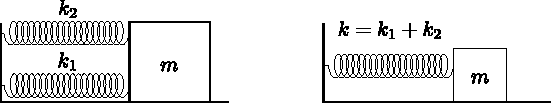
\includegraphics{figures/hlidtenging-gormar.pdf}
\end{figure}
\end{tcolorbox}

\textbf{Útleiðsla:} Við höfum þá að kraftajafnan er gefin með:
\begin{align*}
    ma = -k_1x - k_2 x = -(k_1+k_2)x = -kx
\end{align*}
Svo við sjáum að kerfið hegðar sér eins og gormur með gormstuðul $k = k_1 + k_2$. \qed

\begin{tcolorbox}
\begin{theorem}
\textbf{(Raðtenging gorma)} Þegar við raðtengjum gorma með gormstuðla $k_1, k_2, \ldots, k_n$ þá hegðar kerfið sér eins og einn gormur með gormstuðul $k_{\text{heild}}$ þar sem:
\begin{align*}
    \frac{1}{k_{\text{heild}}} = \frac{1}{k_1} + \frac{1}{k_2} + \ldots + \frac{1}{k_n}.
\end{align*}
\end{theorem}
\begin{figure}[H]
    \centering
    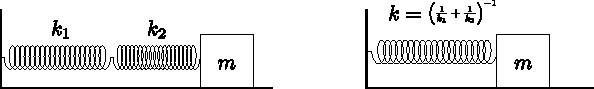
\includegraphics{figures/radtengdir-gormar.pdf}
\end{figure}
\end{tcolorbox}

\textbf{Útleiðsla:} Látum $x_1$ vera strekkinguna á fyrri gorminum og $x_2$ vera strekkinguna á seinni gorminum. Þá er $x = x_1 + x_2$ heildarstrekking kerfisins frá jafnvægisstöðu. Á massann $m$ verkar eininungis gormkraftur frá seinni gorminum svo:
\begin{align*}
    ma = -k_2x_2
\end{align*}
En við vitum þar að auki að $k_1x_1 = k_2x_2$ því togkrafturinn í seinni gorminum hlítur að vera núll því gormurinn er massalaus og einu kraftarnir sem verka á gorminn eru $k_1x_1$ og $k_2x_2$. En þá er:
\begin{align*}
   ma = -kx = -k(x_1 + x_2) = -k\left(-\frac{ma}{k_1} - \frac{ma}{k_2}\right) = k\left( \frac{1}{k_1} + \frac{1}{k_2}  \right)ma \implies \frac{1}{k} = \frac{1}{k_1} + \frac{1}{k_2}.
\end{align*}
\qed

\subsection*{Þéttar}

\begin{tcolorbox}
\begin{theorem}
\textbf{(Hliðtenging þétta)} Þegar að við hliðtengjum þétta með rýmd $C_1, C_2, \ldots, C_n$, þá hegðar kerfið sér eins og kerfi með einu jafngildum þétti með rýmd
\begin{align*}
    C_{\text{heild}} = C_1 + C_2 + \ldots + C_n
\end{align*}
\end{theorem}
\begin{figure}[H]
    \centering
\begin{circuitikz}
      \draw (0,0)
      to[battery1,l=$V$] (0,2)
      to[short] (2,2)
      to[C=$C_1$] (2,0)
      to[short] (0,0);
      \draw (2,2)
      to[short] (4,2)
      to[C=$C_2$] (4,0)
      to[short] (2,0);
    \draw [->] (5.25,1) -- (6.25,1);
    \draw (7.5, 2) 
        to (9.5, 2) 
        to[C=$C_{\text{heild}}\,{=}\,C_1 + C_2$] (9.5, 0)
        to (7.5, 0)
        to[battery1, l=$V$] (7.5, 2);
\end{circuitikz}
\end{figure}
\end{tcolorbox}

\textbf{Útleiðsla:} Samkvæmt lykkjulögmáli Kirchoffs þá þarf spennufallið yfir sérhverja lokaða rás í rásinni að vera núll. Við skoðum því fyrst eftirfarandi lykkju:
\begin{figure}[H]
    \centering
\begin{circuitikz}
      \draw (0,0)
      to[battery1,l=$V$] (0,2)
      to[short] (2,2)
      to[C=$C_1$] (2,0)
      to[short] (0,0);
      \draw (2,2)
      to[short] (4,2)
      to[C=$C_2$] (4,0)
      to[short] (2,0);
      \draw[thin, <-, >=triangle 45,path picture={
            \node[anchor=center]  at (path picture bounding box.center) {$1$};
            }] (1.25,0.5) arc (-60:170:0.4);
\end{circuitikz}
\end{figure}

En þar með sjáum við að $V - \frac{Q_1}{C_1} = 0$ svo $V = \frac{Q_1}{C_1}$. Athugum síðan að ef við skoðum eftirfarandi lykkju:

\begin{figure}[H]
    \centering
\begin{circuitikz}
      \draw (0,0)
      to[battery1,l=$V$] (0,2)
      to[short] (2,2)
      to[C,a=$C_1$] (2,0)
      to[short] (0,0);
      \draw (2,2)
      to[short] (4,2)
      to[C, l=$C_2$] (4,0)
      to[short] (2,0);
      \draw[thin, <-, >=triangle 45,path picture={
            \node[anchor=center]  at (path picture bounding box.center) {$2$};
            }] (3.25,0.5) arc (-60:170:0.4);
\end{circuitikz}
\end{figure}
Þá höfum við að $\frac{Q_2}{C_2} - \frac{Q_1}{C_1} = 0$ svo $\frac{Q_2}{C_2} = \frac{Q_1}{C_1} = V$. Loks skulum við skoða jafngildu rásina:

\begin{figure}[H]
    \centering
\begin{circuitikz}
    \draw (7.5, 2) 
        to (9.5, 2) 
        to[C=$C_{\text{heild}}$] (9.5, 0)
        to (7.5, 0)
        to[battery1, l=$V$] (7.5, 2);
      \draw[thin, <-, >=triangle 45,path picture={
            \node[anchor=center]  at (path picture bounding box.center) {$3$};
            }] (8.75,0.5) arc (-60:170:0.4);
\end{circuitikz}
\end{figure}
En þá höfum við samkvæmt lykkjulögmáli Kirchoffs að $V - \frac{Q_{\text{heild}}}{C_{\text{heild}}} = 0$ svo
\begin{align*}
    C_{\text{heild}} = \frac{Q_{\text{heild}}}{V} = \frac{Q_1 + Q_2}{V} = \frac{C_1 V + C_2 V}{V} = C_1 + C_2.
\end{align*}





\qed

\begin{tcolorbox}
\begin{theorem}
\textbf{(Raðtenging þétta)} Þegar að við raðtengjum þétta með rýmd $C_1, C_2, \ldots, C_n$, þá hegðar kerfið sér eins og kerfi með einu jafngildum þétti með rýmd, $C_{\text{heild}}$, þar sem: 
\begin{align*}
    \frac{1}{C_{\text{heild}}} = \frac{1}{C_1} + \frac{1}{C_2} + \ldots + \frac{1}{C_n}.
\end{align*}
\end{theorem}
\begin{figure}[H]
\centering
\begin{circuitikz}[american voltages]
    \ctikzset{resistors/scale=0.75}
    \draw (0, 2) 
        to[C=$C_1$] (3.5, 2) 
        to (3.5, 0)
        to[C=$C_2$] (0, 0)
        to[battery1, l=$V$] (0, 2);
    \draw [->] (4.5,1) -- (5.5,1);
    \draw (7, 2) 
        to (9, 2) 
        to[C=$C_{\text{heild}}\,{=}\, \left(\frac{1}{C_1} + \frac{1}{C_2}\right)^{-1}$] (9, 0)
        to (7, 0)
        to[battery1, l=$V$] (7, 2);
 \end{circuitikz}
 \end{figure}
\end{tcolorbox}

\textbf{Útleiðsla:} Samkvæmt lykkjulögmáli Kirchoffs er:
\begin{align*}
    V - \frac{Q_1}{C_1} - \frac{Q_2}{C_2} = 0
\end{align*}
Ásamt
\begin{align*}
    V - \frac{Q_{\text{heild}}}{C_{\text{heild}}} = 0.
\end{align*}
En þar sem að rásin er hliðtengd þá er $Q_{\text{heild}} = Q_1 = Q_2$ svo við ályktum að:
\begin{align*}
    \frac{1}{C_{\text{heild}}} = \frac{V}{Q_{\text{heild}}} = \frac{\frac{Q_1}{C_1} + \frac{Q_2}{C_2}}{Q_{\text{heild}}} = \frac{1}{C_1} + \frac{1}{C_2}.
\end{align*}

\qed

\subsection*{Viðnám}

\begin{tcolorbox}
\begin{theorem}
\textbf{(Hliðtenging viðnáma)} Þegar að við hliðtengjum viðnám $R_1, R_2, \ldots, R_n$, þá hegðar kerfið sér eins og kerfi með einu jafngildu viðnámi, $R_{\text{heild}}$, þar sem: 
\begin{align*}
    \frac{1}{R_{\text{heild}}} = \frac{1}{R_1} + \frac{1}{R_2} + \ldots + \frac{1}{R_n}.
\end{align*}
\end{theorem}
\begin{figure}[H]
    \centering
\begin{circuitikz}
      \draw (0,0)
      to[battery1,l=$V$] (0,2)
      to[short] (2,2)
      to[R=$R_1$] (2,0)
      to[short] (0,0);
      \draw (2,2)
      to[short] (4,2)
      to[R=$R_2$] (4,0)
      to[short] (2,0);
    \draw [->] (5,1) -- (6,1);
    \draw (7.5, 2) 
        to (9.5, 2) 
        to[R=$R_{\text{heild}}\,{=}\,\left(\frac{1}{R_1} + \frac{1}{R_2}\right)^{-1}$] (9.5, 0)
        to (7.5, 0)
        to[battery1, l=$V$] (7.5, 2);
\end{circuitikz}
\end{figure}
\end{tcolorbox}

\textbf{Útleiðsla:} Með því að skoða lykkjurnar þá fáum við að:
\begin{align*}
    V = R_1 I_1 = R_2 I_2 = R_{\text{heild}} I_{\text{heild}}
\end{align*}
Þar að auki sjáum við ef við notum gatnamótalögmál Kirchoffs að $I = I_1 + I_2$. En þar með er:
\begin{align*}
    \frac{1}{R_{\text{heild}}} = \frac{I_{\text{heild}}}{V} = \frac{I_1 + I_2}{V} = \frac{\frac{V}{R_1} + \frac{V}{R_2}}{V} = \frac{1}{R_1} + \frac{1}{R_2}.
\end{align*}

\qed

\begin{tcolorbox}
\begin{theorem}
\textbf{(Raðtenging viðnáma)} Þegar við raðtengjum viðnám, $R_1, R_2, \ldots, R_n$, þá heðgar kerfið sér eins og kerfi með einu jafngildu viðnámi
\begin{align*}
    R_{\text{heild}} = R_1 + R_2 + \ldots + R_n
\end{align*}
\end{theorem}
\begin{figure}[H]
\centering
\begin{circuitikz}[american voltages]
    \ctikzset{resistors/scale=0.75}
    \draw (0, 2) 
        to[R=$R_1$] (3.5, 2) 
        to (3.5, 0)
        to[R=$R_2$] (0, 0)
        to[battery1, l=$V$] (0, 2);
    \draw [->] (4.5,1) -- (5.5,1);
    \draw (7, 2) 
        to (9, 2) 
        to[R=$R_{\text{heild}}\,{=}\,R_1 + R_2$] (9, 0)
        to (7, 0)
        to[battery1, l=$V$] (7, 2);
 \end{circuitikz}
 \end{figure}
\end{tcolorbox}

\textbf{Útleiðsla:} Við höfum þá samkvæmt lykkjulögmáli Kirchoffs að:
\begin{align*}
    V - IR_1 - IR_2 = 0
\end{align*}
En í jafngildu rásinni væri $V = I R_{\text{heild}}$ svo við ályktum að $R_{\text{heild}} = R_1 + R_2$.

\qed

\subsection*{Spólur}

\begin{tcolorbox}
\begin{theorem} 
\textbf{(Hliðtenging spóla)} Þegar við hliðtengjum spólur með spanstuðla, $L_1, L_2, \ldots, L_n$, þá heðgar kerfið sér eins og kerfi með einni jafngildri spólu með spanstuðul $L_{\text{heild}}$ þar sem
\begin{align*}
    \frac{1}{L_{\text{heild}}} = \frac{1}{L_1} + \frac{1}{L_2} + \ldots + \frac{1}{L_n}.
\end{align*}
\end{theorem}
\begin{figure}[H]
    \centering
\begin{circuitikz}
      \draw (0,0)
      to[battery1,l=$V$] (0,2)
      to[short] (2,2)
      to[L=$L_1$] (2,0)
      to[short] (0,0);
      \draw (2,2)
      to[short] (4,2)
      to[L=$L_2$] (4,0)
      to[short] (2,0);
    \draw [->] (5.25,1) -- (6.25,1);
    \draw (7.5, 2) 
        to (9.5, 2) 
        to[L=$L_{\text{heild}}\,{=}\,\left(\frac{1}{L_1} + \frac{1}{L_2}\right)^{-1}$] (9.5, 0)
        to (7.5, 0)
        to[battery1, l=$V$] (7.5, 2);
\end{circuitikz}
\end{figure}
\end{tcolorbox}

\textbf{Útleiðsla:} Samkvæmt lykkjulögmáli Kirchoffs þá er:
\begin{align*}
    V - L_1 \dot{I}_1 = 0, \hspace{0.5cm} V - L_2 \dot{I}_2 = 0, \hspace{0.5cm} V - L_{\text{heild}} \dot{I} = 0.
\end{align*}

Þar sem að heildarstraumurinn sem að flæðir í rásinni er $I = I_1 + I_2$ þá er $\dot{I} = \dot{I}_1 + \dot{I}_2$ með því að diffra. Við ályktum því að:
\begin{align*}
    \frac{1}{L_{\text{heild}}} = \frac{\dot{I}}{V} = \frac{\dot{I}_1 + \dot{I}_2}{V} = \frac{\frac{V}{L_1} + \frac{V}{L_2}}{V} = \frac{1}{L_1} + \frac{1}{L_2}.
\end{align*}

\qed


\begin{tcolorbox}
\begin{theorem}
\textbf{(Raðtenging spóla)} Þegar við raðtengjum spólur með spanstuðla, $L_1, L_2, \ldots, L_n$, þá hegðar kerfið sér eins og kerfi með einni jafngildri spólu með spanstuðul
\begin{align*}
    L_{\text{heild}} = L_1 + L_2 + \ldots + L_n
\end{align*}
\end{theorem}
\begin{figure}[H]
\centering
\begin{circuitikz}[american voltages]
    \ctikzset{resistors/scale=0.75}
    \draw (0, 2) 
        to[L=$L_1$] (3.5, 2) 
        to (3.5, 0)
        to[L=$L_2$] (0, 0)
        to[battery1, l=$V$] (0, 2);
    \draw [->] (4.5,1) -- (5.5,1);
    \draw (7, 2) 
        to (9, 2) 
        to[L=$L_{\text{heild}}\,{=}\,L_1 + L_2$] (9, 0)
        to (7, 0)
        to[battery1, l=$V$] (7, 2);
 \end{circuitikz}
 \end{figure}

\end{tcolorbox}

\textbf{Útleiðsla:} Við höfum samkvæmt lykkjulögmálinu að:
\begin{align*}
    V - L_1 \dot{I} - L_2 \dot{I} = 0 = V - L_{\text{heild}}\dot{I} \implies  L_{\text{heild}} = L_1 + L_2.
\end{align*}

\qed

\section{Drude-líkanið (*)}

Í þessum viðauka munum við reyna að útskýra einfalt líkan fyrir rafstraum. Það er nefnilega svolítið skrítið að við gerum ráð fyrir að rafstraumurinn sé fastur í rásinni þ.e.a.s.~að rafeindirnar ferðist með jöfnum hraða í gegnum rafrásina. Því ef við rifjum upp tengslin milli rafspennu og rafsviðs, $\Delta V = Ed$ þá sjáum við að rafeindirnar ættu að finna fyrir rafsviði, $E$, og þar með rafkrafti $F_E = eE$, en þar með myndu þær hafa fasta hröðun, $a = \frac{eE}{m}$, í rásinni og rafstraumurinn ætti að aukast eftir því sem að rafeindirnar ferðast lengra í rásinni. Við munum nú reyna að útskýra hvers vegna rafeindirnar ferðast með jöfnum hraða í rásinni. Hliðstæðu er að finna í loftmótsstöðu og lokahraðanum sem að hlutir ná í frjálsu falli með loftmótsstöðu. \\

\vspace{0.2cm}


Við skoðum vírbút af lengd $\ell$ með þverskurðarflatarmál $A$ sem að samanstendur af efni með heildarmassa $M$ og mólmassa $\mu$. Látum spennumuninn á milli enda vírbútsins vera $\Delta V$ og þar með er rafsviðið í vírbútnum gefið með $E = \frac{\Delta V}{\ell}$. 

\begin{figure}[H]
    \centering
    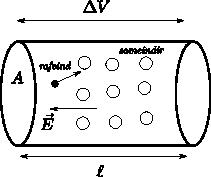
\includegraphics[scale = 1.4]{figures/drude1.pdf}
\end{figure}

Við lítum á sem svo að rafeindirnar séu á hreyfingu en að sameindirnar séu kyrrstæðar og að rafeindirnar skoppi á milli sameindanna og lendi í árekstrum við þær. Vegna rafsviðsins finna rafeindirnar fyrir krafti $F_E = eE$ en í árekstrunum við sameindirnar þá finna þær fyrir einhversskonar loftmótsstöðu:
\begin{align*}
    F_{\text{árekstur}} = \frac{\Delta p}{\Delta t}
\end{align*}
þar sem að $\Delta p$ er skriðþungabreytingin á tímanum $\Delta t$. Látum $\tau$ tákna meðaltímann sem líður á milli árekstra rafeindanna við sameindirnar (við munum síðar sýna hvernig er hægt að ákvarða $\tau$). Þegar að rafeindirnar skoppa af sameindunum með hraða $v$ þá geta þær fengið hvaða hraða sem er á bilinu $[-v,v]$ svo að meðaltali er hraði rafeindanna eftir áreksturinn $0$ (sumar hafa þá neikvæðan hraða en aðrar jákvæðan en að meðaltali hafa þær engan hraða eftir áreksturinn). En það þýðir að skriðþungabreytingin á milli 
árekstra verður að meðaltali:
\begin{align*}
    F_{\text{árekstur}} = \frac{\Delta p}{\Delta t} = \frac{mv - m \cdot 0}{\tau} = \frac{mv}{\tau}
\end{align*}
En þar með verður heildarkraftajafnan:
\begin{align*}
    ma = eE - \frac{mv}{\tau}
\end{align*}
Í kraftajafnvægi er $a = 0$ og þá ferðast rafeindirnar þess vegna með föstum hraða sem kallast rekhraði:
\begin{align*}
    0 = ma = eE - \frac{mv}{\tau} \implies v_d = \frac{eE}{m}\tau.
\end{align*}
Látum nú $f_e$ tákna heildarfjölda rafeinda á rúmmálseiningu. Þá verður rafstraumurinn:
\begin{align*}
    I = \frac{\Delta q}{\Delta t} = \frac{e \cdot f_e \cdot A v_d \tau}{\tau} = e f_e A v_d = \frac{e^2 f_e \tau}{m} A E.
\end{align*}

Við skilgreinum þá eðlisviðnám sem stærðina:
\begin{align*}
    \rho = \frac{m}{e^2 f_e \tau}
\end{align*}
Þá höfum við sýnt að:
\begin{align*}
    I = \frac{A}{\rho} E
\end{align*}
Viðnámið var síðan skilgreint sem stærðin $R = \frac{\rho L}{A}$ svo að við höfum hér sýnt að:
\begin{align*}
    I = \frac{A }{\rho} E = \frac{E \ell}{R}
\end{align*}
En $E \ell = \Delta V$ svo við ályktum að $\Delta V = E \ell = IR$. Þar með höfum við leitt út lögmál Ohms. \\

\newpage

\section{Dæmi}

\subsection*{Dæmatími 13: Jafngildir þéttar}

\begin{tcolorbox}
\begin{figure}[H]
\centering
\begin{circuitikz}[american voltages]
    \ctikzset{capacitors/scale=0.75}
    \draw (0, 2) 
        to[C=$C_1$] (2,2) to[C=$C_2$] (4, 2) 
        to (4, 0)
        to (0, 0)
        to[battery1, l=$V$] (0, 2);
    \draw [->] (4.5,1) -- (5.5,1);
    \draw (4,1.4) node[label={[font=\footnotesize]\emph{Raðtenging}}] {};
    \draw (7, 2) 
        to (9, 2) 
        to[C=$C_{\text{heild}}\,{=}\,\left(\frac{1}{C_1} + \frac{1}{C_2}\right)^{-1}$] (9, 0)
        to (7, 0)
        to[battery1, l=$V$] (7, 2);
 \end{circuitikz}
\end{figure}
\begin{figure}[H]
    \centering
\begin{circuitikz}
    \ctikzset{resistors/scale=0.75}
      \draw (0,0)
      to[battery1,l=$V$] (0,2)
      to[short] (2,2)
      to[C=$C_1$] (2,0)
      to[short] (0,0);
      \draw (2,2)
      to[short] (4,2)
      to[C=$C_2$] (4,0)
      to[short] (2,0);
    \draw [->] (5,1) -- (6,1);
    \draw (7.5, 2) 
        to (9.5, 2)
        to[C=$C_{\text{heild}}\,{=}\,C_1 + C_2$] (9.5, 0)
        to (7.5, 0)
        to[battery1, l=$V$] (7.5, 2);
        \draw (4.5,1.4) node[label={[font=\footnotesize]\emph{Hliðtenging}}] {};
\end{circuitikz}
\end{figure}
\end{tcolorbox}

\begin{enumerate}[label = \textbf{(\alph*)}]

\item[\textbf{(26.27 og 26.28)}] Einfaldið eftirfarandi rásir og ákvarðið heildarrýmdir þeirra:

\begin{figure}[H]
    \centering
    \begin{circuitikz}[american voltages]
    \ctikzset{capacitors/scale=0.75}
    \draw (0, 2) to[battery1=\,, a=$V$] (0,0) to (3,0) to[C=\SI{20}{\mu F}] (3,1) to (4,1) to (4,2) to[C=$\SI{10}{\mu F}$] (0,2);
    \draw (3,0) to (5,0) to[C=\SI{10}{\mu F}] (5,1) to (4,1);
    \draw (7,2) to[battery1=\,, a=$V$] (7,0) to (9.5,0) to[C=\SI{30}{\mu F}] (9.5,1) to[C=\SI{20}{\mu F}] (9.5,2) to (7,2);
    \draw (9.5,0) to (11,0) to[C, a=\SI{13}{\mu F}] (11,2) to (9.5,2);
 \end{circuitikz}
\end{figure}

\item[\textbf{(26.56 og 26.57)}] Ákvarðið hleðsluna og spennufallið yfir hvern þétti í rásunum hér fyrir neðan:

\begin{figure}[H]
    \centering
    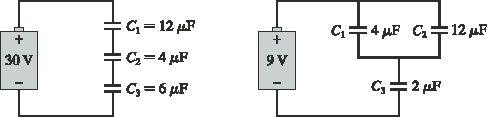
\includegraphics[scale = 1.25]{figures/rk2653.pdf}
\end{figure}

\begin{tcolorbox}
\begin{enumerate*}[label = \vspace{0.1cm}]
  \item \textbf{(26.27)} $C_{\text{heild}} = \SI{7.5}{\mu F}$.
  \item \textbf{(26.28)} $C_{\text{heild}} = \SI{25}{\mu F}$. \\
  \item \textbf{(26.56)} $Q = \SI{60}{\mu C}, \Delta V_1 = \SI{5}{V}, \Delta V_2 = \SI{15}{V}, \Delta V_3 = \SI{10}{V}$. \\
  \item \textbf{(26.57)} $Q = \SI{16}{\mu C}, Q_1 = \SI{4}{\mu C}, Q_2 = \SI{12}{\mu C}, Q_3 = \SI{16}{\mu C}$.
\end{enumerate*}
\end{tcolorbox}



\end{enumerate}

\newpage

\subsection*{Dæmatími 14: Jafngild viðnám}

\begin{tcolorbox}
\begin{figure}[H]
\centering
\begin{circuitikz}[american voltages]
    \ctikzset{resistors/scale=0.75}
    \draw (0, 2) 
        to[R=$R_1$] (2,2) to[R=$R_2$] (4, 2) 
        to (4, 0)
        to (0, 0)
        to[battery1, l=$V$] (0, 2);
    \draw [->] (4.5,1) -- (5.5,1);
    \draw (4,1.4) node[label={[font=\footnotesize]\emph{Raðtenging}}] {};
    \draw (7, 2) 
        to (9, 2) 
        to[R=$R_{\text{heild}}\,{=}\,R_1 + R_2$] (9, 0)
        to (7, 0)
        to[battery1, l=$V$] (7, 2);
 \end{circuitikz}
\end{figure}
\begin{figure}[H]
    \centering
\begin{circuitikz}
    \ctikzset{resistors/scale=0.75}
      \draw (0,0)
      to[battery1,l=$V$] (0,2)
      to[short] (2,2)
      to[R=$R_1$] (2,0)
      to[short] (0,0);
      \draw (2,2)
      to[short] (4,2)
      to[R=$R_2$] (4,0)
      to[short] (2,0);
    \draw [->] (5,1) -- (6,1);
    \draw (7.5, 2) 
        to (9.5, 2)
        to[R=$R_{\text{heild}}\,{=}\,\left(\frac{1}{R_1} + \frac{1}{R_2}\right)^{-1}$] (9.5, 0)
        to (7.5, 0)
        to[battery1, l=$V$] (7.5, 2);
        \draw (4.5,1.4) node[label={[font=\footnotesize]\emph{Hliðtenging}}] {};
\end{circuitikz}
\end{figure}
\end{tcolorbox}

\begin{enumerate}[label = \textbf{(\alph*)}]

\item[\textbf{(28.25 og 28.26)}] Einfaldið eftirfarandi rásir og ákvarðið heildarviðnám þeirra:

\begin{figure}[H]
    \centering
    \begin{circuitikz}[american voltages]
    \ctikzset{resistors/scale=0.5}
    \ctikzset{capacitors/scale=0.5}
    \draw (1, 4) to[battery1=\,, a=$V$] (1,0) to[R,l=\SI{10}{\ohm}] (4,0) to (4,0.5) to (5,0.5) to[R,a=\SI{20}{\ohm}] (5,2) to[R,a=\SI{55}{\ohm}] (5,3.5) to (4,3.5) to (4,4) to (1,4);
    \draw (4,0.5) to (3,0.5) to[R,a=\SI{40}{\ohm}] (3,2) to[R,a=\SI{10}{\ohm}] (3,3.5) to (4,3.5);
    \draw (8, 5) to[battery1=\,, a=$V$] (8,0) to (12,0) to (12,0.5) to (12.5,0.5) to[R,a=\SI{30}{\ohm}] (12.5,2.5) to[R,a=\SI{5}{\ohm}] (12.5,4.5) to (12,4.5) to (12,5) to (8,5);
    \draw (12,4.5) to (10,4.5) to (10, 4);
    \draw (9.5,4) to (10.5,4);
    \draw (9.5,4) to[R,a=\SI{12}{\ohm}] (9.5,3) to (10.5,3);
    \draw (10.5,4) to[R,l=\SI{24}{\ohm}] (10.5,3);
    \draw (10,3) to (10,2.5);
    \draw (9,2.5) to (11,2.5);
    \draw (11,2.5) to[R,l=\SI{20}{\ohm}] (11,0.5);
    \draw (9,2.5) to[R,l=\SI{10}{\ohm}] (9,0.5);
    \draw (10,2.5) to[R,l=\SI{60}{\ohm}] (10,0.5);
    \draw (9,0.5) to (12,0.5);
 \end{circuitikz}
\end{figure}

\item[\textbf{(28.58 og 28.59)}] Ákvarðið rafstrauminn og spennufallið yfir hvert viðnám í rásunum hér fyrir neðan:

\begin{figure}[H]
    \centering
    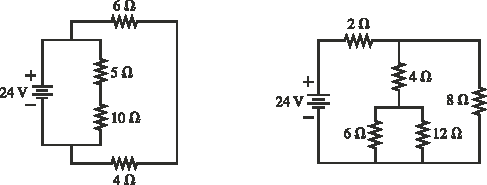
\includegraphics[scale = 1.25]{figures/rk2856.pdf}
\end{figure}

\end{enumerate}

\begin{tcolorbox}
\begin{enumerate*}[label = ]
  \item \textbf{(28.25)} $R_{\text{heild}} = \SI{40}{\ohm}$.
  \item \textbf{(28.26)} $R_{\text{heild}} = \SI{10}{\ohm}$.
  \item \textbf{(28.58)} $I = \SI{4.0}{A}, I_1 = \SI{2.4}{A}, I_2 = \SI{1.6}{A}$. \\
  \item \textbf{(28.59)} $I = \SI{4.0}{A}, I_1 = I_2 = \SI{2.0}{A}, I_3 = \SI{1.33}{A}, I_4 = \SI{0.67}{A}$.
\end{enumerate*}
\end{tcolorbox}

\newpage

\subsection*{Dæmatími 15: Lögmál Kirchoffs}

\begin{tcolorbox}
Lykkjulögmál Kirchoffs segir að heildarspennufallið við það að fara hring í rafrás er núll. Með öðrum orðum: $\Delta V_{\text{heild}} = \Delta V_1 + \Delta V_2 + \ldots + \Delta V_n = 0$. Gatnamótalögmál Kirchoffs segir að ef að $I_{\text{inn}}$ er heildarrafstraumurinn sem flæðir inn í punkt og $I_{\text{út}}$ er heildarrafstraumurinn sem flæðir út úr sama punkti þá er $I_{\text{inn}} = I_{\text{út}}$. Spennuföllin eru:
\begin{align*}
    \Delta V_R = IR, \hspace{0.9cm} \Delta V_C = \frac{Q}{C}, \hspace{0.9cm} \Delta V_L = L \dot{I} = L \frac{dI}{dt}.
\end{align*}
\end{tcolorbox}

\begin{enumerate}[label = \textbf{(\alph*)}]

\item[\textbf{(28.4)}] Hver er stærð og stefna straumsins sem fer í gegnum \SI{10}{\ohm} viðnámið á myndinni hér fyrir neðan?

\begin{figure}[H]
    \centering
    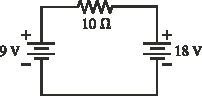
\includegraphics[scale = 1.2]{figures/rk284.pdf}
\end{figure}

\item[\textbf{(28.31)}] Hver er spennumunurinn, $\Delta V  = V_b - V_a$ milli punktanna $a$ og $b$ á myndinni hér fyrir neðan?

\begin{figure}[H]
    \centering
    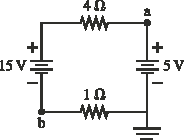
\includegraphics[scale = 1.2]{figures/rk2831.pdf}
\end{figure}

\item[\textbf{(28.52)}] Straummælirinn á myndinni hér fyrir neðan sýnir $\SI{3.0}{A}$. Ákvarðið $\mathcal{E}, I_1$ og $I_2$. 

\begin{figure}[H]
    \centering
    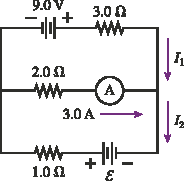
\includegraphics[scale = 1.2]{figures/rk2852.pdf}
\end{figure}

\item[\textbf{(28.63)}] Hver er stærð og stefna straumsins sem fer í gegnum \SI{10}{\ohm} viðnámið á myndinni hér fyrir neðan?

\begin{figure}[H]
    \centering
    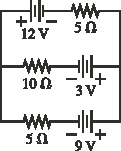
\includegraphics[scale = 1.2]{figures/rk2863.pdf}
\end{figure}

\end{enumerate}

\begin{tcolorbox}
\begin{enumerate*}[label = ]
  \item \textbf{(28.4)} $I = \SI{0.9}{A}$.
  \item \textbf{(28.31)} $\Delta V = -\SI{7.0}{V}$.
  \item \textbf{(28.52)} $\mathcal{E} = \SI{12}{V}, I_1 = \SI{3.0}{A}$.
  \item \textbf{(28.63)} $I = \SI{0.45}{A}$.
\end{enumerate*}
\end{tcolorbox}

\newpage

\subsection*{Dæmatími 16: Afl í rafrásum}

\begin{tcolorbox}
Varmaaflið/rafaflið sem tapast í rafrásum er gefið með:
\begin{align*}
    P = \frac{dE}{dt} = \frac{d\left(qV \right)}{dt} = \frac{dq}{dt}V = IV.
\end{align*}
Þar sem $V$ táknar spennufallið yfir tiltekinn íhlut og $I$ táknar rafstrauminn í gegnum íhlutinn.
\end{tcolorbox}


\begin{enumerate}[label = \textbf{(\alph*)}]

\item[\textbf{(28.7)}] Í hefðbundnum innstungum hér á landi notum við \SI{220}{V} riðspennu sem sveiflast með $\SI{50}{Hz}$ tíðni. Dyson Supersonic hárblásari notar \SI{1600}{W} stafrænan mótor til þess að gefa nákvæman og öflugan blástur. Hversu mikill straumur er í Dyson Supersonic hárblásaranum þegar hann er í gangi? Hvert þarf innra viðnámið í hárblásarnum að vera?

\item[\textbf{(28.8)}] Lítum á myndina hér fyrir neðan til vinstri. Hversu mikið rafafl tapast út um hvort viðnám?

\begin{figure}[H]
    \centering
    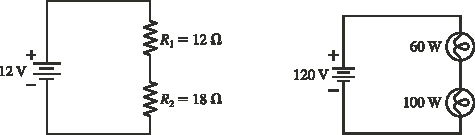
\includegraphics[scale = 1.25]{figures/rk288.pdf}
\end{figure}

\item[\textbf{(28.9)}] Lítum á myndina hér fyrir ofan til hægri. Búið er að koma fyrir tveimur ljósaperum fyrir í rásinni, einni \SI{60}{W} og einni \SI{100}{W}. Athugið að ljósaperur hafa innra viðnám og styrkur ljósaperu ákvarðast út frá aflinu sem að peran myndi gefa ef að hún væri tengd við \SI{220}{V} heimilisspennu. Báðar ljósaperurnar skína. Hvor ljósaperan skín skærar og hversu mikið rafafl tapast í hvorri ljósaperu?

\item[\textbf{(28.78)}] Hvert er rafaflið sem tapast í gegnum \SI{2}{\ohm} viðnámið á myndinni hér fyrir neðan?

\begin{figure}[H]
    \centering
    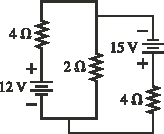
\includegraphics[scale = 1.25]{figures/rk2873.pdf}
\end{figure}

\end{enumerate}

\begin{tcolorbox}
\begin{enumerate*}[label = \vspace{0.1cm}]
  \item \textbf{(28.7)} $I = \SI{7.3}{A}, R = \SI{30}{\ohm}$.
  \item \textbf{(28.8)} $P_1 = \SI{1.9}{W} > P_2 = \SI{2.9}{W}$. 
  \item \textbf{(28.9)} $P_1 = \SI{7.0}{W} > P_2 = \SI{4.2}{W}$. 
  \item \textbf{(28.78)} $P = \SI{0.29}{W}$.
\end{enumerate*}
\end{tcolorbox}

\newpage

\subsection*{Dæmatími 17: Eðlisviðnám}

\begin{tcolorbox}
Viðnám víra er breytilegt eftir því úr hvaða efni þeir eru gerðir. Almennt gildir að viðnám vírsins er:
\begin{align*}
    R = \rho \frac{\ell}{A}.
\end{align*}
Þar sem $\rho$ er eðlisviðnám vírsins, $\ell$ er lengd vírsins og $A$ er þverskurðarflatarmál hans.
\begin{table}[H]
    \centering
    \begin{tabular}{|l|c|}
    \hline
        \textbf{Efni} & \textbf{Eðlisviðnám} \\ \hline \hline
        Ál & \SI{2.8e-8}{\ohm.m}  \\ \hline
        Kopar & \SI{1.7e-8}{\ohm.m} \\ \hline
        Gull & \SI{2.4e-8}{\ohm.m} \\ \hline
        Járn & \SI{9.7e-8}{\ohm.m} \\ \hline
        Silfur & \SI{1.6e-8}{\ohm.m} \\ \hline
        Volfram & \SI{5.6e-8}{\ohm.m} \\ \hline
        Nikkel & \SI{1.5e-6}{\ohm.m} \\ \hline
        Kolefni & \SI{3.5e-5}{\ohm.m} \\ \hline
    \end{tabular}
\end{table}
\end{tcolorbox}

\begin{enumerate}[label = \textbf{(\alph*)}]

\item[\textbf{(27.27)}] \textbf{(a)} Hvert er viðnám gullvírs sem er \SI{2.0}{m} á lengd og hefur þvermál \SI{0.20}{mm}. \textbf{(b)} Hvert er viðnám rétthyrningslaga kolefnisvírs sem hefur hliðarlengdir $\SI{1.0}{mm}$ og lengd $\SI{10}{cm}$? 

\item[\textbf{(27.28)}] Verkfræðingur tekur \SI{94}{cm} langan vír sem hefur þvermál $\SI{0.33}{mm}$ og tengir hann við rafhlöðu með \SI{1.5}{V} spennu. Með því að nota straummæli sér hann að straumurinn í rásinni er \SI{8.0}{A}. Úr hvaða efni er vírinn?

\item[\textbf{(27.33)}] Blýið í blýöntum er í alvörunni úr kolefni. Blýantur af lengd $\SI{6.0}{cm}$ og með \SI{0.70}{mm} þvermál er tengdur í sitthvorn endann við \SI{9.0}{V} rafhlöðu. Hver er straumurinn sem að fer í gegnum blýantinn?

\item[\textbf{(27.37)}] Rafmagnsvírarnir sem eru notaðir í rafrásum heimila eru oftast koparvírar með þvermál \SI{2.0}{mm}. Vírarnir geta þurft að vera mjög langir í stórum íbúðarhúsum til þess að ná að tengja allt sem þarf að tengja. Hver er spennumunurinn á milli endanna á \SI{20}{m} löngum heimilisvír sem ber \SI{8.0}{A} rafstraum?

\end{enumerate}

\begin{tcolorbox}
\begin{enumerate*}[label = \vspace{0.1cm}]
  \item \textbf{(27.27)} $R_{\!_{\text{Au}}} = \SI{1.5}{\ohm}, R_{\!_{\text{C}}} = \SI{3.5}{\ohm}$.
  \item \textbf{(27.28)} \text{Silfri}.
  \item \textbf{(27.33)} $I = \SI{1.6}{A}$.
  \item \textbf{(27.37)} $\Delta V = \SI{0.87}{V}$.
\end{enumerate*}
\end{tcolorbox}

\newpage